% PP-Article.tex for AEA last revised 22 June 2011
\documentclass[twocolumn, a4paper]{article}

%%%%%% NOTE FROM OVERLEAF: The mathtime package is no longer publicly available nor distributed. We recommend using a different font package e.g. mathptmx if you'd like to use a Times font.
\usepackage{mathptmx}
\usepackage{amsmath}
\usepackage[dutch]{babel}
\usepackage{subcaption}
\usepackage[width=.8\textwidth]{caption}
\usepackage{float}
\usepackage{booktabs}
\usepackage{multicol}
\usepackage{longtable}
\usepackage{minted}
% If you have trouble with the mathtime package please see our technical support 
% document at: http://www.aeaweb.org/templates/technical_support.pdf
% You may remove the mathtime package if you can't get it working but your page
% count may be inaccurate as a result.
% \usepackage[cmbold]{mathtime}
\usepackage{xargs}                      % Use more than one optional parameter in a new commands 
\usepackage[pdftex,dvipsnames]{xcolor}  % Coloured text etc.
% 
\usepackage{pdfpages}
\usepackage[colorinlistoftodos,prependcaption,textsize=tiny]{todonotes}
\newcommandx{\unsure}[2][1=]{\todo[linecolor=red,backgroundcolor=red!25,bordercolor=red,#1]{#2}}
\setlength{\marginparwidth}{2cm}
% Note: you may use either harvard or natbib (but not both) to provide a wider
% variety of citation commands than latex supports natively. See below.

% Uncomment the next line to use the natbib package with bibtex 
%\usepackage{natbib}
\usepackage{titlesec}

\titlespacing*\section{0pt}{12pt plus 4pt minus 2pt}{0pt plus 2pt minus 2pt}
\titlespacing*\subsection{0pt}{12pt plus 4pt minus 2pt}{0pt plus 2pt minus 2pt}
\titlespacing*\subsubsection{0pt}{12pt plus 4pt minus 2pt}{0pt plus 2pt minus 2pt}



% Uncomment the next line to use the harvard package with bibtex
%\usepackage[abbr]{harvard}

% This command determines the leading (vertical space between lines) in draft mode
% with 1.5 corresponding to "double" spacing.
\begin{document}

\title{Geavanceerde computerarchitectuur: Labo 01 \\ 
\large{Array omwisselen}}
\author{\textsc{Anton Danneels en Pieter Delobelle}}
\date{}
\maketitle

\section{Inleiding}
Het doel van dit labo is om een array om te draaien, zowel op de CPU alsook de GPU van de computer. 
Hierdoor moet een inzicht bekomen worden over het performantieverschil dat een GPU kan bieden ten opzichte van een CPU; en in welke situaties dit verschil naar boven komt.

Deze opdracht wordt ge\"implementeerd op een grafische kaart van NVIDEA, waarbij het \emph{CUDA}-framework gebruikt kan worden. 

\section{Analyse}

\subsection{GPU}
Een GPU bestaat uit vele CUDA-cores, bedoeld om een \emph{single instruction multiple thread} (SIMT) architectuur te ondersteunen. Deze cores zijn verdeeld over een aantal \emph{stream multiprocessors} (SM), welke ook weer opgedeeld zijn in een aantal \emph{wraps}. Deze wraps kunnen typisch 32 threads in parallel runnen, waardoor de blocksize idealiter een veelvoud van 32 is.

\subsection{CUDA}
Om de taken van de threads effici\"ent te kunnen verdelen, biedt CUDA een \emph{grid} aan. Dit grid bestaat uit blokken, die dus uitgevoerd worden door een SM. Binnen deze blokken kunnen threads ge\"identificeerd worden door een 1D, 2D of 3D set van indices. In ieder geval, de grootte $x \cdot y \cdot z$ kan niet groter zijn dan het aantal threads op een SM.

Om dit op te lossen, zijn blokken ook ge-indexed, waarbij een queue wordt aangelegd door de GPU. Om de algemene index te bepalen, wordt de volgende code gebruikt (voor 1 dimensie): 

\begin{minted}{c}
  int i = blockIdx.x * blockDim.x 
    + threadIdx.x;
\end{minted}
\label{c:index}

\subsection{XOR-verwisseling}
Om de waarden te swappen, wordt gebruikt gemaakt van het \emph{XOR swapping algoritme}. Dit werkt als volgt:

\begin{minted}{c}
  X = X XOR Y
  Y = Y XOR X
  X = X XOR Y
\end{minted}

Het resultaat zijn twee variabelen die van waarde zijn verwisseld, zonder gebruik te maken van een helper-variabele.

\section{Oplossing}
Om de GPU en CPU te kunnen vergelijken, is de code om een array te swappen twee keer ge\"implementeerd: eenmaal voor de CPU met een traditionele for-lus en eenmaal voor de GPU, waarbij met variabele blocksize.

Daarnaast is ook de lengte van de array variabel, waardoor de evaluatie over meerdere lengtes kan gebeuren. De code hiervoor is te vinden als bijlage.

\begin{figure*}
  \centering
  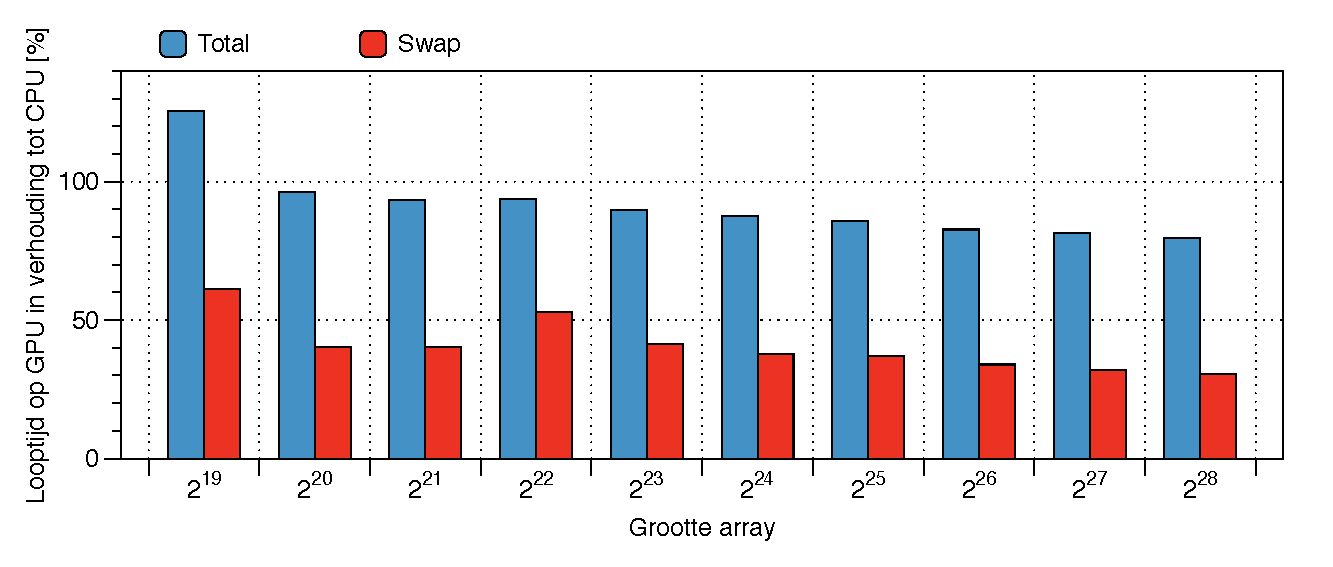
\includegraphics[width=0.8\textwidth]{cpu_vs_gpu.eps}
  \caption{Eerste experiment, de vergelijking tussen CPU en GPU voor verschillende array-groottes met een blocksize $n=64$}
  \label{fig:b4_cpu_gpu}
\end{figure*}

\subsection{Swap op de CPU}
Voor de array om te wisselen op de CPU, itereren we tot het midden van de array, waarbij beide helften worden omgewisseld.

\begin{minted}{console}
  0000,0001,0002,0003,0004,0005
  0005,0004,0003,0002,0001,0000 
  Operation in 0 ms
\end{minted}

Om de performantie te vergelijken, benchmarken we deze operatie ook. Dit doen we voor de CPU door \mintinline{c}{clock()} twee maal op te roepen. Deze klok heeft technisch gezien een precisie van 1 ns, dus de variabele \mintinline{c}{CLOCKS_PER_SEC} = 1 000 000. Door een geheelgetallige afronding is de precisie van onze meting afgekapt op 1 ms. Voor kleine arrays is dit niet ideaal.

Deze timing is onderverdeeld in de tijd nodig om de array te initialiseren en de daadwerkelijke tijd nodig om de wisseling uit te voeren.

\subsection{Swap op de GPU}
De swap-operatie op de GPU is inhoudelijk gelijk, maar de lus is vervangen door functie in sectie~\ref{c:index} om de index te bepalen. Deze c

De benchmarks worden bij CUDA niet gemeten via de \mintinline{c}{clock()}-functie, aangezien we er niet vanuit mogen gaan dat de code op de GPU niet gesynchroniseerd hoeft te zijn. CUDA biedt echter ook een functie aan, waarmee de tijd als zwevende kommagetal kan gemeten worden. 

\begin{minted}{c}
  cudaEventRecord(swap_start);
  cudaEventSynchronize(swap_stop);
  cudaEventElapsedTime( &ms, 
    swap_start, 
    swap_stop );
\end{minted}
 
Zoals bij de CPU, vergelijken we zowel de daadwerkelijke operatie alsook de tijd die nodig is om de array te initialiseren én bijkomend ook te kopieren naar het geheugen op de videokaart.

In het eerste experiment, dat te zien is op figuur~\ref{fig:b4_cpu_gpu}, is de blocksize $n$ vast gedefineerd, terwijl iteratief een range van array-groottes wordt ge\"evalueerd. De resultaten hiervan---en ook de tweede test--- zijn ook te vinden in de bijlagen.

Een tweede experiment richt specifiek op de blocksize, waarvan de resultaten in figuur~\ref{blocksize} zijn weergegeven. Ter vergelijking is ook de CPU-tijd gevisualiseerd. 

\subsection{Vergelijking}
De resultaten van het eerste experiment in figuur ~\ref{fig:b4_cpu_gpu} vergelijken de swap- en totale tijden tussen de CPU en GPU. Hierbij is de CPU als baseline (100 \%) genomen.

Uit de data valt duidelijk op te maken dat de GPU sneller is voor

In figuur~\ref{blocksize} is de invloed van de grootte van de blocksize op de uitvoersnelheid weergegeven. Ter vergelijking is ook de tijd op de CPU weergegeven.

\begin{figure}
\centering
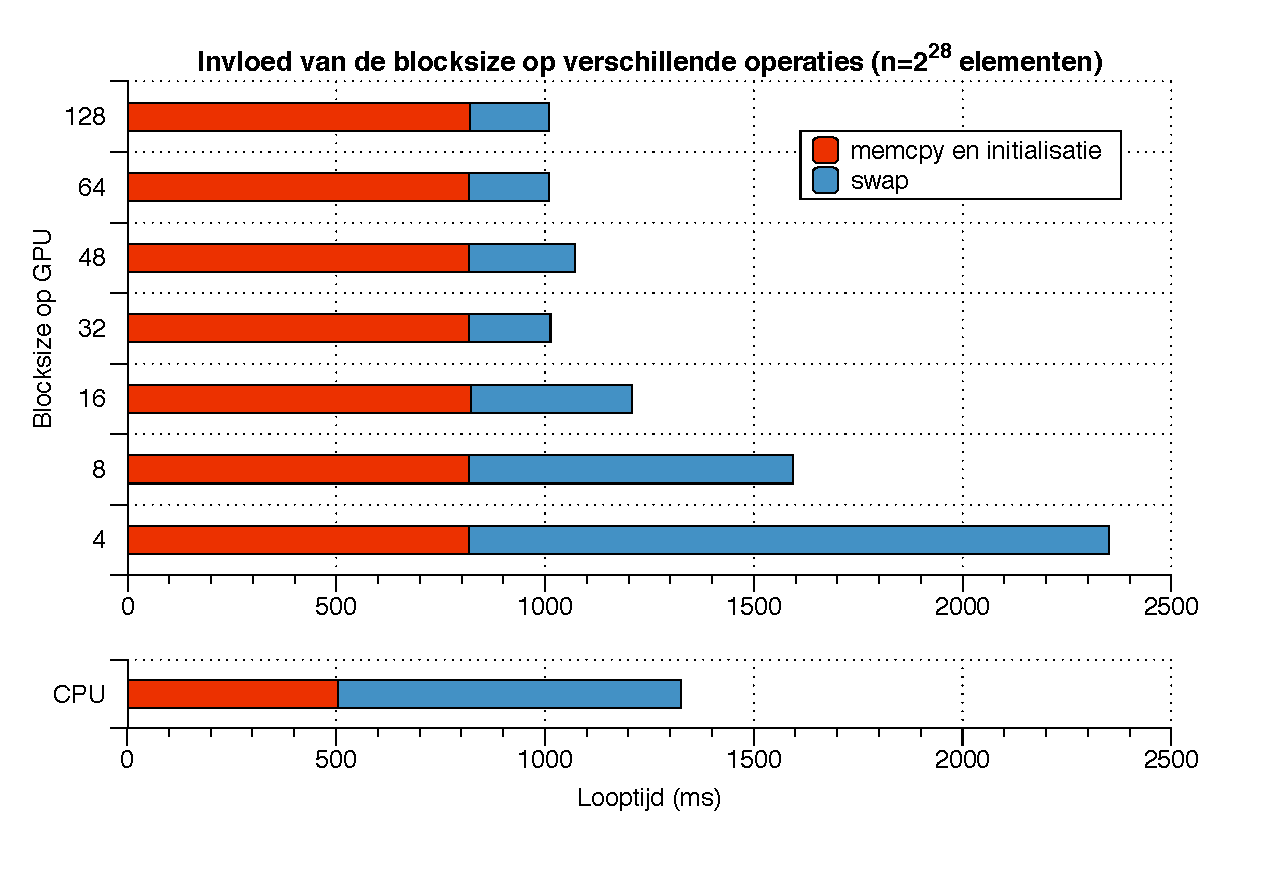
\includegraphics[width=0.55\textwidth]{blocksize.eps}
\caption{Invloed van de blocksize op de uitvoersnelheid.}
\label{blocksize}
\end{figure}

Uit de grafiek is duidelijk op te maken dat blocksizes $n$ die een veelvoud zijn van 32 een overduidelijk sneller zijn. Hoe beter de wraps benut worden---door dus veelvouden van 32 te kiezen, hoe beter de uitvoersnelheid is. Door deze zeer ongelukkig te kiezen, zien we zelfs dat de resultaten zelfs slechter zijn 

\begin{figure}
  \centering
  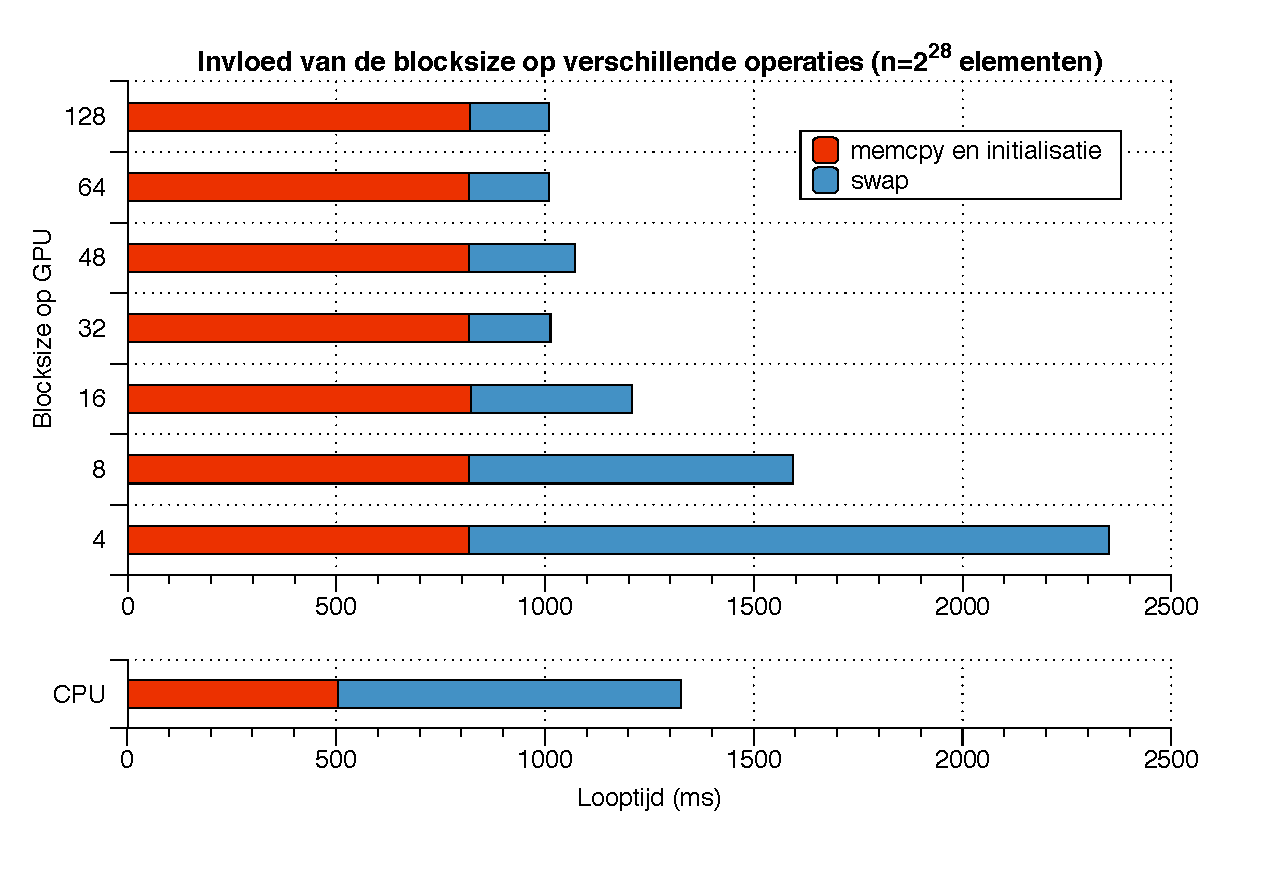
\includegraphics[width=0.55\textwidth]{blocksize.eps}
  \caption{Invloed van de blocksize op de uitvoersnelheid.}
  \label{blocksize}
  \end{figure}

\section{Besluit}
Zoals verwacht is de gpu sneller

Block size impact

Overhead bij upload/download


\onecolumn

\appendix

\begin{figure}[H]
  \centering
  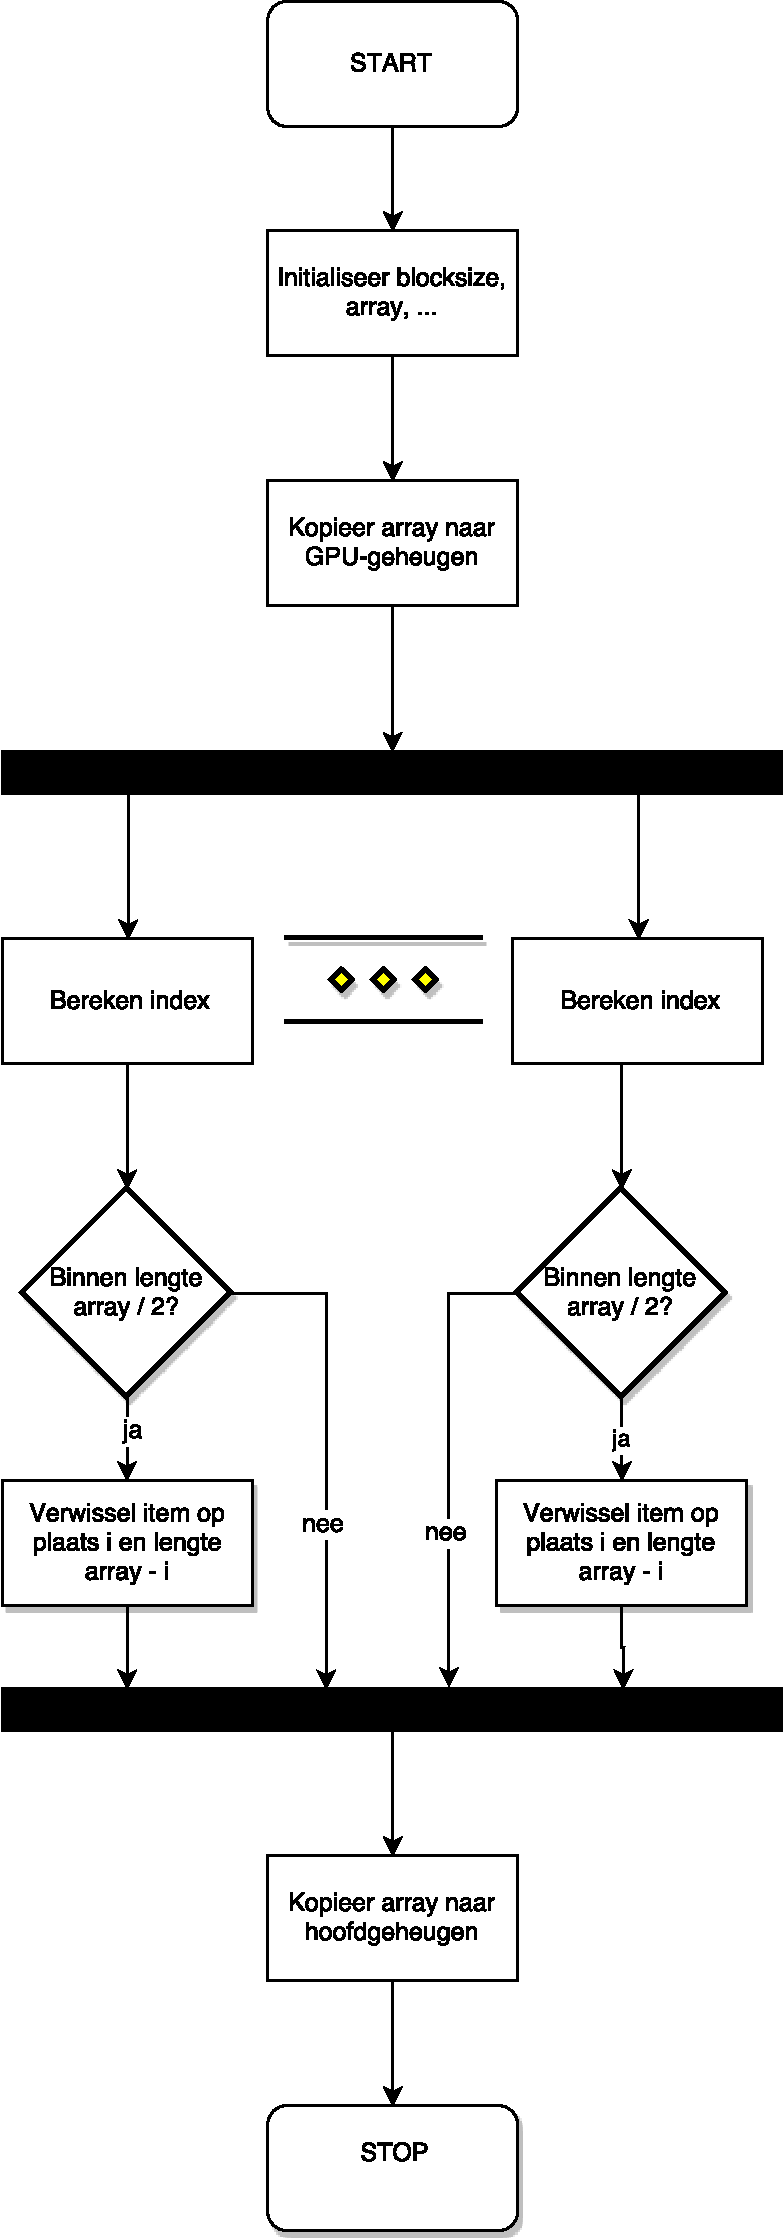
\includegraphics[width=0.4\textwidth]{flowgraph.pdf}
  \caption{Flowchart van de code om de array te swappen op de GPU.}
\end{figure}

\newpage

% Please add the following required packages to your document preamble:
% \usepackage{booktabs}
% \usepackage{longtable}
% Note: It may be necessary to compile the document several times to get a multi-page table to line up properly
\begin{longtable}[c]{@{}rrrrrrrr@{}}
    \caption{My caption}
    \label{my-label}\\
    \toprule
    blocksize & n         & cpu\_swap & cpu\_tot & gpu\_swap   & 2\textasciicircum n & gpu\_tot    & gpu\_delta \\* \midrule
    \endfirsthead
    %
    \multicolumn{8}{c}%
    {{\bfseries Table \thetable\ continued from previous page}} \\
    \toprule
    blocksize & n         & cpu\_swap & cpu\_tot & gpu\_swap   & 2\textasciicircum n & gpu\_tot    & gpu\_delta \\* \midrule
    \endhead
    %
    \bottomrule
    \endfoot
    %
    \endlastfoot
    %
    4         & 1         & 0         & 0        & 0.026720    & 0                   & 0.231104    & 0.204384   \\
    4         & 2         & 0         & 0        & 0.016000    & 1                   & 0.166656    & 0.150656   \\
    4         & 4         & 0         & 0        & 0.015136    & 2                   & 0.157184    & 0.142048   \\
    4         & 8         & 0         & 0        & 0.015136    & 3                   & 0.154304    & 0.139168   \\
    4         & 16        & 0         & 0        & 0.015328    & 4                   & 0.153184    & 0.137856   \\
    4         & 32        & 0         & 0        & 0.015104    & 5                   & 0.152416    & 0.137312   \\
    4         & 64        & 0         & 0        & 0.014528    & 6                   & 0.152352    & 0.137824   \\
    4         & 128       & 0         & 0        & 0.015232    & 7                   & 0.151872    & 0.13664    \\
    4         & 256       & 0         & 0        & 0.015680    & 8                   & 0.153824    & 0.138144   \\
    4         & 512       & 0         & 0        & 0.017248    & 9                   & 0.156480    & 0.139232   \\
    4         & 1024      & 0         & 0        & 0.019648    & 10                  & 0.160800    & 0.141152   \\
    4         & 2048      & 0         & 0        & 0.026048    & 11                  & 0.171136    & 0.145088   \\
    4         & 4096      & 0         & 0        & 0.039392    & 12                  & 0.192640    & 0.153248   \\
    4         & 8192      & 0         & 0        & 0.066496    & 13                  & 0.237408    & 0.170912   \\
    4         & 16384     & 0         & 0        & 0.123200    & 14                  & 0.330976    & 0.207776   \\
    4         & 32768     & 0         & 0        & 0.235488    & 15                  & 0.793952    & 0.558464   \\
    4         & 65536     & 0         & 0        & 0.460480    & 16                  & 5.750496    & 5.290016   \\
    4         & 131072    & 0         & 0        & 0.908800    & 17                  & 1.840640    & 0.93184    \\
    4         & 262144    & 0         & 1        & 1.960640    & 18                  & 3.293632    & 1.332992   \\
    4         & 524288    & 1         & 3        & 3.763616    & 19                  & 5.953568    & 2.189952   \\
    4         & 1048576   & 3         & 6        & 7.537440    & 20                  & 11.550176   & 4.012736   \\
    4         & 2097152   & 6         & 10       & 15.129824   & 21                  & 22.104416   & 6.974592   \\
    4         & 4194304   & 13        & 22       & 30.214945   & 22                  & 43.626751   & 13.411806  \\
    4         & 8388608   & 25        & 42       & 59.756802   & 23                  & 86.269539   & 26.512737  \\
    4         & 16777216  & 51        & 83       & 107.737984  & 24                  & 160.028442  & 52.290458  \\
    4         & 33554432  & 104       & 169      & 192.220093  & 25                  & 297.628571  & 105.408478 \\
    4         & 67108864  & 207       & 337      & 383.706909  & 26                  & 589.636902  & 205.929993 \\
    4         & 134217728 & 411       & 665      & 765.873962  & 27                  & 1176.011108 & 410.137146 \\
    4         & 268435456 & 822       & 1326     & 1532.069702 & 28                  & 2350.672119 & 818.602417 \\
    8         & 1         & 0         & 0        & 0.026720    & 0                   & 0.231104    & 0.204384   \\
    8         & 2         & 0         & 0        & 0.016000    & 1                   & 0.166656    & 0.150656   \\
    8         & 4         & 0         & 0        & 0.015136    & 2                   & 0.157184    & 0.142048   \\
    8         & 8         & 0         & 0        & 0.015136    & 3                   & 0.154304    & 0.139168   \\
    8         & 16        & 0         & 0        & 0.015328    & 4                   & 0.153184    & 0.137856   \\
    8         & 32        & 0         & 0        & 0.015104    & 5                   & 0.152416    & 0.137312   \\
    8         & 64        & 0         & 0        & 0.014528    & 6                   & 0.152352    & 0.137824   \\
    8         & 128       & 0         & 0        & 0.015232    & 7                   & 0.151872    & 0.13664    \\
    8         & 256       & 0         & 0        & 0.015680    & 8                   & 0.153824    & 0.138144   \\
    8         & 512       & 0         & 0        & 0.017248    & 9                   & 0.156480    & 0.139232   \\
    8         & 1024      & 0         & 0        & 0.019648    & 10                  & 0.160800    & 0.141152   \\
    8         & 2048      & 0         & 0        & 0.026048    & 11                  & 0.171136    & 0.145088   \\
    8         & 4096      & 0         & 0        & 0.039392    & 12                  & 0.192640    & 0.153248   \\
    8         & 8192      & 0         & 0        & 0.066496    & 13                  & 0.237408    & 0.170912   \\
    8         & 16384     & 0         & 0        & 0.123200    & 14                  & 0.330976    & 0.207776   \\
    8         & 32768     & 0         & 0        & 0.235488    & 15                  & 0.793952    & 0.558464   \\
    8         & 65536     & 0         & 0        & 0.460480    & 16                  & 5.750496    & 5.290016   \\
    8         & 131072    & 0         & 0        & 0.908800    & 17                  & 1.840640    & 0.93184    \\
    8         & 262144    & 0         & 1        & 1.960640    & 18                  & 3.293632    & 1.332992   \\
    8         & 524288    & 1         & 3        & 3.763616    & 19                  & 5.953568    & 2.189952   \\
    8         & 1048576   & 3         & 6        & 7.537440    & 20                  & 11.550176   & 4.012736   \\
    8         & 2097152   & 6         & 10       & 15.129824   & 21                  & 22.104416   & 6.974592   \\
    8         & 4194304   & 13        & 22       & 30.214945   & 22                  & 43.626751   & 13.411806  \\
    8         & 8388608   & 25        & 42       & 59.756802   & 23                  & 86.269539   & 26.512737  \\
    8         & 16777216  & 51        & 83       & 107.737984  & 24                  & 160.028442  & 52.290458  \\
    8         & 33554432  & 104       & 169      & 192.220093  & 25                  & 297.628571  & 105.408478 \\
    8         & 67108864  & 207       & 337      & 383.706909  & 26                  & 589.636902  & 205.929993 \\
    8         & 134217728 & 411       & 665      & 765.873962  & 27                  & 1176.011108 & 410.137146 \\
    8         & 268435456 & 822       & 1326     & 1532.069702 & 28                  & 2350.672119 & 818.602417 \\
    16        & 1         & 0         & 0        & 0.026112    & 0                   & 0.212128    & 0.186016   \\
    16        & 2         & 0         & 0        & 0.015552    & 1                   & 0.163392    & 0.14784    \\
    16        & 4         & 0         & 0        & 0.014752    & 2                   & 0.154528    & 0.139776   \\
    16        & 8         & 0         & 0        & 0.014464    & 3                   & 0.151776    & 0.137312   \\
    16        & 16        & 0         & 0        & 0.015296    & 4                   & 0.180224    & 0.164928   \\
    16        & 32        & 0         & 0        & 0.014592    & 5                   & 0.158784    & 0.144192   \\
    16        & 64        & 0         & 0        & 0.014400    & 6                   & 0.158816    & 0.144416   \\
    16        & 128       & 0         & 0        & 0.014272    & 7                   & 0.176992    & 0.16272    \\
    16        & 256       & 0         & 0        & 0.014368    & 8                   & 0.147488    & 0.13312    \\
    16        & 512       & 0         & 0        & 0.015232    & 9                   & 0.150240    & 0.135008   \\
    16        & 1024      & 0         & 0        & 0.016448    & 10                  & 0.152800    & 0.136352   \\
    16        & 2048      & 0         & 0        & 0.018784    & 11                  & 0.159200    & 0.140416   \\
    16        & 4096      & 0         & 0        & 0.024192    & 12                  & 0.171392    & 0.1472     \\
    16        & 8192      & 0         & 0        & 0.037280    & 13                  & 0.201152    & 0.163872   \\
    16        & 16384     & 0         & 0        & 0.066144    & 14                  & 0.258336    & 0.192192   \\
    16        & 32768     & 0         & 0        & 0.122656    & 15                  & 0.376064    & 0.253408   \\
    16        & 65536     & 0         & 0        & 0.234016    & 16                  & 0.581184    & 0.347168   \\
    16        & 131072    & 0         & 0        & 0.455616    & 17                  & 1.135360    & 0.679744   \\
    16        & 262144    & 0         & 1        & 0.905600    & 18                  & 1.980800    & 1.0752     \\
    16        & 524288    & 1         & 2        & 1.835616    & 19                  & 3.714080    & 1.878464   \\
    16        & 1048576   & 3         & 5        & 3.770400    & 20                  & 7.434112    & 3.663712   \\
    16        & 2097152   & 6         & 10       & 7.340992    & 21                  & 14.347904   & 7.006912   \\
    16        & 4194304   & 13        & 21       & 15.054016   & 22                  & 28.770657   & 13.716641  \\
    16        & 8388608   & 25        & 41       & 29.408833   & 23                  & 56.575710   & 27.166877  \\
    16        & 16777216  & 52        & 83       & 58.803905   & 24                  & 110.853729  & 52.049824  \\
    16        & 33554432  & 103       & 166      & 117.574974  & 25                  & 221.985474  & 104.4105   \\
    16        & 67108864  & 205       & 332      & 202.782425  & 26                  & 409.763397  & 206.980972 \\
    16        & 134217728 & 410       & 663      & 387.181702  & 27                  & 796.707947  & 409.526245 \\
    16        & 268435456 & 822       & 1327     & 774.899963  & 28                  & 1592.852417 & 817.952454 \\
    32        & 1         & 0         & 0        & 0.026304    & 0                   & 0.222464    & 0.19616    \\
    32        & 2         & 0         & 0        & 0.016640    & 1                   & 0.185024    & 0.168384   \\
    32        & 4         & 0         & 0        & 0.014720    & 2                   & 0.154112    & 0.139392   \\
    32        & 8         & 0         & 0        & 0.014208    & 3                   & 0.181440    & 0.167232   \\
    32        & 16        & 0         & 0        & 0.014336    & 4                   & 0.177856    & 0.16352    \\
    32        & 32        & 0         & 0        & 0.014656    & 5                   & 0.158048    & 0.143392   \\
    32        & 64        & 0         & 0        & 0.014592    & 6                   & 0.158752    & 0.14416    \\
    32        & 128       & 0         & 0        & 0.014688    & 7                   & 0.157952    & 0.143264   \\
    32        & 256       & 0         & 0        & 0.014176    & 8                   & 0.157536    & 0.14336    \\
    32        & 512       & 0         & 0        & 0.023808    & 9                   & 0.180256    & 0.156448   \\
    32        & 1024      & 0         & 0        & 0.014528    & 10                  & 0.161664    & 0.147136   \\
    32        & 2048      & 0         & 0        & 0.015968    & 11                  & 0.166720    & 0.150752   \\
    32        & 4096      & 0         & 0        & 0.017696    & 12                  & 0.182112    & 0.164416   \\
    32        & 8192      & 0         & 0        & 0.022496    & 13                  & 0.187392    & 0.164896   \\
    32        & 16384     & 0         & 0        & 0.037312    & 14                  & 0.231520    & 0.194208   \\
    32        & 32768     & 0         & 0        & 0.066176    & 15                  & 0.350176    & 0.284      \\
    32        & 65536     & 0         & 0        & 0.122432    & 16                  & 0.471936    & 0.349504   \\
    32        & 131072    & 0         & 0        & 0.233632    & 17                  & 0.789696    & 0.556064   \\
    32        & 262144    & 0         & 1        & 0.458528    & 18                  & 1.472128    & 1.0136     \\
    32        & 524288    & 1         & 2        & 0.924256    & 19                  & 2.858368    & 1.934112   \\
    32        & 1048576   & 3         & 5        & 1.948992    & 20                  & 5.999584    & 4.050592   \\
    32        & 2097152   & 6         & 10       & 3.675776    & 21                  & 10.638464   & 6.962688   \\
    32        & 4194304   & 12        & 21       & 8.781536    & 22                  & 22.679840   & 13.898304  \\
    32        & 8388608   & 25        & 42       & 16.280865   & 23                  & 43.810944   & 27.530079  \\
    32        & 16777216  & 52        & 84       & 29.393312   & 24                  & 82.480515   & 53.087203  \\
    32        & 33554432  & 104       & 168      & 59.686562   & 25                  & 164.604218  & 104.917656 \\
    32        & 67108864  & 207       & 333      & 107.966850  & 26                  & 313.733124  & 205.766274 \\
    32        & 134217728 & 413       & 665      & 193.956741  & 27                  & 604.857605  & 410.900864 \\
    32        & 268435456 & 823       & 1329     & 386.880005  & 28                  & 1209.285767 & 822.405762 \\
    48        & 1         & 0         & 0        & 0.024352    & 0                   & 0.203904    & 0.179552   \\
    48        & 2         & 0         & 0        & 0.015008    & 1                   & 0.168512    & 0.153504   \\
    48        & 4         & 0         & 0        & 0.014016    & 2                   & 0.162432    & 0.148416   \\
    48        & 8         & 0         & 0        & 0.014208    & 3                   & 0.160384    & 0.146176   \\
    48        & 16        & 0         & 0        & 0.014112    & 4                   & 0.236672    & 0.22256    \\
    48        & 32        & 0         & 0        & 0.014560    & 5                   & 0.162560    & 0.148      \\
    48        & 64        & 0         & 0        & 0.014112    & 6                   & 0.160960    & 0.146848   \\
    48        & 128       & 0         & 0        & 0.014624    & 7                   & 0.187328    & 0.172704   \\
    48        & 256       & 0         & 0        & 0.014656    & 8                   & 0.164448    & 0.149792   \\
    48        & 512       & 0         & 0        & 0.014976    & 9                   & 0.160960    & 0.145984   \\
    48        & 1024      & 0         & 0        & 0.014848    & 10                  & 0.162624    & 0.147776   \\
    48        & 2048      & 0         & 0        & 0.015232    & 11                  & 0.167040    & 0.151808   \\
    48        & 4096      & 0         & 0        & 0.016096    & 12                  & 0.175808    & 0.159712   \\
    48        & 8192      & 0         & 0        & 0.016160    & 13                  & 0.182944    & 0.166784   \\
    48        & 16384     & 0         & 0        & 0.022400    & 14                  & 0.216576    & 0.194176   \\
    48        & 32768     & 0         & 0        & 0.037568    & 15                  & 0.280800    & 0.243232   \\
    48        & 65536     & 0         & 0        & 0.067936    & 16                  & 0.238176    & 0.17024    \\
    48        & 131072    & 0         & 0        & 0.123136    & 17                  & 0.680448    & 0.557312   \\
    48        & 262144    & 0         & 1        & 0.236832    & 18                  & 1.290016    & 1.053184   \\
    48        & 524288    & 1         & 2        & 0.470592    & 19                  & 2.380192    & 1.9096     \\
    48        & 1048576   & 3         & 5        & 0.933216    & 20                  & 4.728096    & 3.79488    \\
    48        & 2097152   & 6         & 10       & 1.853792    & 21                  & 8.841728    & 6.987936   \\
    48        & 4194304   & 13        & 22       & 3.697664    & 22                  & 17.433249   & 13.735585  \\
    48        & 8388608   & 25        & 42       & 8.022368    & 23                  & 35.602783   & 27.580415  \\
    48        & 16777216  & 53        & 84       & 14.867776   & 24                  & 68.187134   & 53.319358  \\
    48        & 33554432  & 103       & 166      & 29.551424   & 25                  & 132.463577  & 102.912153 \\
    48        & 67108864  & 205       & 331      & 59.075008   & 26                  & 264.489380  & 205.414372 \\
    48        & 134217728 & 410       & 663      & 101.647873  & 27                  & 511.711060  & 410.063187 \\
    48        & 268435456 & 821       & 1325     & 195.260696  & 28                  & 1012.969238 & 817.708542 \\
    64        & 1         & 0         & 0        & 0.030528    & 0                   & 0.271072    & 0.240544   \\
    64        & 2         & 0         & 0        & 0.157792    & 1                   & 0.325760    & 0.167968   \\
    64        & 4         & 0         & 0        & 0.014368    & 2                   & 0.164512    & 0.150144   \\
    64        & 8         & 0         & 0        & 0.016064    & 3                   & 0.189952    & 0.173888   \\
    64        & 16        & 0         & 0        & 0.014048    & 4                   & 0.564256    & 0.550208   \\
    64        & 32        & 0         & 0        & 0.016672    & 5                   & 0.169472    & 0.1528     \\
    64        & 64        & 0         & 0        & 0.015424    & 6                   & 0.155520    & 0.140096   \\
    64        & 128       & 0         & 0        & 0.015296    & 7                   & 0.150720    & 0.135424   \\
    64        & 256       & 0         & 0        & 0.014816    & 8                   & 0.149440    & 0.134624   \\
    64        & 512       & 0         & 0        & 0.014048    & 9                   & 0.150624    & 0.136576   \\
    64        & 1024      & 0         & 0        & 0.014336    & 10                  & 0.151456    & 0.13712    \\
    64        & 2048      & 0         & 0        & 0.014976    & 11                  & 0.155552    & 0.140576   \\
    64        & 4096      & 0         & 0        & 0.016608    & 12                  & 0.164320    & 0.147712   \\
    64        & 8192      & 0         & 0        & 0.018880    & 13                  & 0.183712    & 0.164832   \\
    64        & 16384     & 0         & 0        & 0.027776    & 14                  & 0.221888    & 0.194112   \\
    64        & 32768     & 0         & 0        & 0.047616    & 15                  & 0.303904    & 0.256288   \\
    64        & 65536     & 0         & 0        & 0.084352    & 16                  & 0.433792    & 0.34944    \\
    64        & 131072    & 0         & 0        & 0.158464    & 17                  & 0.710656    & 0.552192   \\
    64        & 262144    & 0         & 1        & 0.308576    & 18                  & 1.361824    & 1.053248   \\
    64        & 524288    & 1         & 2        & 0.611680    & 19                  & 2.511168    & 1.899488   \\
    64        & 1048576   & 3         & 5        & 1.213408    & 20                  & 4.807776    & 3.594368   \\
    64        & 2097152   & 6         & 10       & 2.416928    & 21                  & 9.344544    & 6.927616   \\
    64        & 4194304   & 12        & 21       & 6.361856    & 22                  & 19.720287   & 13.358431  \\
    64        & 8388608   & 25        & 41       & 10.310720   & 23                  & 36.748512   & 26.437792  \\
    64        & 16777216  & 51        & 82       & 19.302591   & 24                  & 71.741600   & 52.439009  \\
    64        & 33554432  & 104       & 168      & 38.599712   & 25                  & 143.883652  & 105.28394  \\
    64        & 67108864  & 207       & 335      & 70.304253   & 26                  & 277.131866  & 206.827613 \\
    64        & 134217728 & 412       & 665      & 131.725540  & 27                  & 541.917847  & 410.192307 \\
    64        & 268435456 & 832       & 1344     & 253.048996  & 28                  & 1070.998413 & 817.949417 \\
    128       & 2         & 0         & 0        & 0.017248    & 1                   & 0.207552    & 0.190304   \\
    128       & 4         & 0         & 0        & 0.016160    & 2                   & 0.199040    & 0.18288    \\
    128       & 8         & 0         & 0        & 0.016160    & 3                   & 0.195264    & 0.179104   \\
    128       & 16        & 0         & 0        & 0.016000    & 4                   & 0.193728    & 0.177728   \\
    128       & 32        & 0         & 0        & 0.016512    & 5                   & 0.194656    & 0.178144   \\
    128       & 64        & 0         & 0        & 0.015776    & 6                   & 0.195552    & 0.179776   \\
    128       & 128       & 0         & 0        & 0.016768    & 7                   & 0.194880    & 0.178112   \\
    128       & 256       & 0         & 0        & 0.016288    & 8                   & 0.195200    & 0.178912   \\
    128       & 512       & 0         & 0        & 0.016256    & 9                   & 0.197152    & 0.180896   \\
    128       & 1024      & 0         & 0        & 0.015904    & 10                  & 0.199072    & 0.183168   \\
    128       & 2048      & 0         & 0        & 0.017600    & 11                  & 0.204096    & 0.186496   \\
    128       & 4096      & 0         & 0        & 0.018336    & 12                  & 0.214816    & 0.19648    \\
    128       & 8192      & 0         & 0        & 0.019488    & 13                  & 0.239008    & 0.21952    \\
    128       & 16384     & 0         & 0        & 0.022496    & 14                  & 0.230880    & 0.208384   \\
    128       & 32768     & 0         & 0        & 0.037728    & 15                  & 0.297472    & 0.259744   \\
    128       & 65536     & 0         & 0        & 0.065792    & 16                  & 0.437600    & 0.371808   \\
    128       & 131072    & 0         & 0        & 0.122912    & 17                  & 0.674944    & 0.552032   \\
    128       & 262144    & 0         & 1        & 0.238368    & 18                  & 1.302016    & 1.063648   \\
    128       & 524288    & 1         & 2        & 0.466976    & 19                  & 2.568128    & 2.101152   \\
    128       & 1048576   & 3         & 5        & 0.915232    & 20                  & 4.718944    & 3.803712   \\
    128       & 2097152   & 6         & 11       & 1.818912    & 21                  & 8.777664    & 6.958752   \\
    128       & 4194304   & 12        & 21       & 5.163584    & 22                  & 18.596512   & 13.432928  \\
    128       & 8388608   & 26        & 41       & 7.805344    & 23                  & 34.176674   & 26.37133   \\
    128       & 16777216  & 51        & 83       & 14.505632   & 24                  & 67.594078   & 53.088446  \\
    128       & 33554432  & 103       & 166      & 28.994144   & 25                  & 131.901794  & 102.90765  \\
    128       & 67108864  & 205       & 333      & 58.011265   & 26                  & 263.177185  & 205.16592  \\
    128       & 134217728 & 410       & 663      & 97.118210   & 27                  & 506.298584  & 409.180374 \\
    128       & 268435456 & 821       & 1324     & 190.015869  & 28                  & 1008.206482 & 818.190613 \\* \bottomrule
    \end{longtable}

\newpage

\inputminted[tabsize=4,obeytabs, ]{c}{main.c}

% The appendix command is issued once, prior to all appendices, if any.
%\appendix
\end{document}

